\documentclass[11pt]{article}

\usepackage{amsmath, amsfonts}
\usepackage{graphicx}
\usepackage{hyperref}
\usepackage{fontspec}
\usepackage{titlesec}
\usepackage{apacite}
\usepackage{csvsimple,longtable,booktabs}

\titlelabel{\thetitle. }

\oddsidemargin 0pt
\evensidemargin 0pt
\marginparwidth 40pt
\marginparsep 10pt
\topmargin -20pt
\headsep 10pt
\textheight 8.7in
\textwidth 6.65in
\linespread{1.2}
\setlength{\parindent}{0cm} % Default is 15pt.

\fontencoding{T1}
\defaultfontfeatures{Mapping=tex-text,Scale=MatchLowercase}
\setmainfont{Palatino}
\setmonofont{PT Mono}

\title{Bivariate analysis of follower count and the average number of likes on Instagram}
\author{Taichi Kato}
\date{May, 2019}

\begin{document}

\maketitle

\begin{abstract}
\textit{
}
\end{abstract}

\section{Introduction}\label{section-introduction}

\quad\quad With the rise of information age came the increase in significance of online presence. 
It is not without a doubt, that especially within the younger generation, prominence of an individual is often evaluated based on their online popularity. 
Furthermore, empirically speaking, such evaluation of individuals based has increased even more in the past few years.
Instagram, being one of the most commonly used social media platforms, boasts more than 1 billion monthly users \cite{techcrunch:online}, displaying its inconceivable popularity.
Instagram is a social media network similar to Facebook, where users share images and engage with other users.
The most common methods of engagement is through "liking", which can be done through tapping the image twice.
It signifies to the poster that the user who has "liked" the content appreciated it.
On Instagram, different users "follow" each other.
When a user follows another user, the content shared by the other user will be shown in the user's timeline called the feed.
Such design of the application engages users to follow others who share content that they like.
Hence, the amount of likes and followers can both be said to signify the content and user's popularity, respectively.
As expected, these numeric values are often used by the younger generations as indicators of an individual's real-life popularity, with many celebrities boasting a large number of followers on Instagram.

However, despite the society's reliance on Instagram engagement and follower count as a metric for the determination of one's success, there has been little research regarding what these values mean, and how they relate to each other.
As an active user of Instagram myself, I was especially interested in the factors which determine the number of likes a user attains, and how these factors are related to each other.
Since the number of likes a user attains is dependent on the number of people who see the user's content, it would be reasonable to hypothesise that the number of followers the user would have will affect the number of likes a user gets. 
Hence, through this exploration, I aim to find the relationship between the average number of likes a user gets and their follower count, in order to determine how exactly these values are related, if at all.

\section{Dataset}\label{section-dataset}

\subsection{Data Collection Method}

\quad\quad In identifying the relationship between the follower count and the number of likes, a comprehensive data about Instagram users are required. The research will start with three randomly chosen "seed" users in which their followers are crawled as well. This will allow for a compilation of a reasonably balanced and diverse data set of users, which can approximate the active user population of Instagram. A crawler written in Python was created, with an array containing all followers of the three seed users, and their user properties, is private, number of likes, verification status, biography url, number of media, profile category, number of followers, and number of following users. The program was ran on a virtual machine and left running for 5 hours. Through this method, a total of 1023 user data was collected. Of those, 875 of the s

The collected data was saved in to a csv file in the following format, with the raw data being available in the Appendix.

\subsection{Data Processing}
\begin{figure}[h!]
  \center
  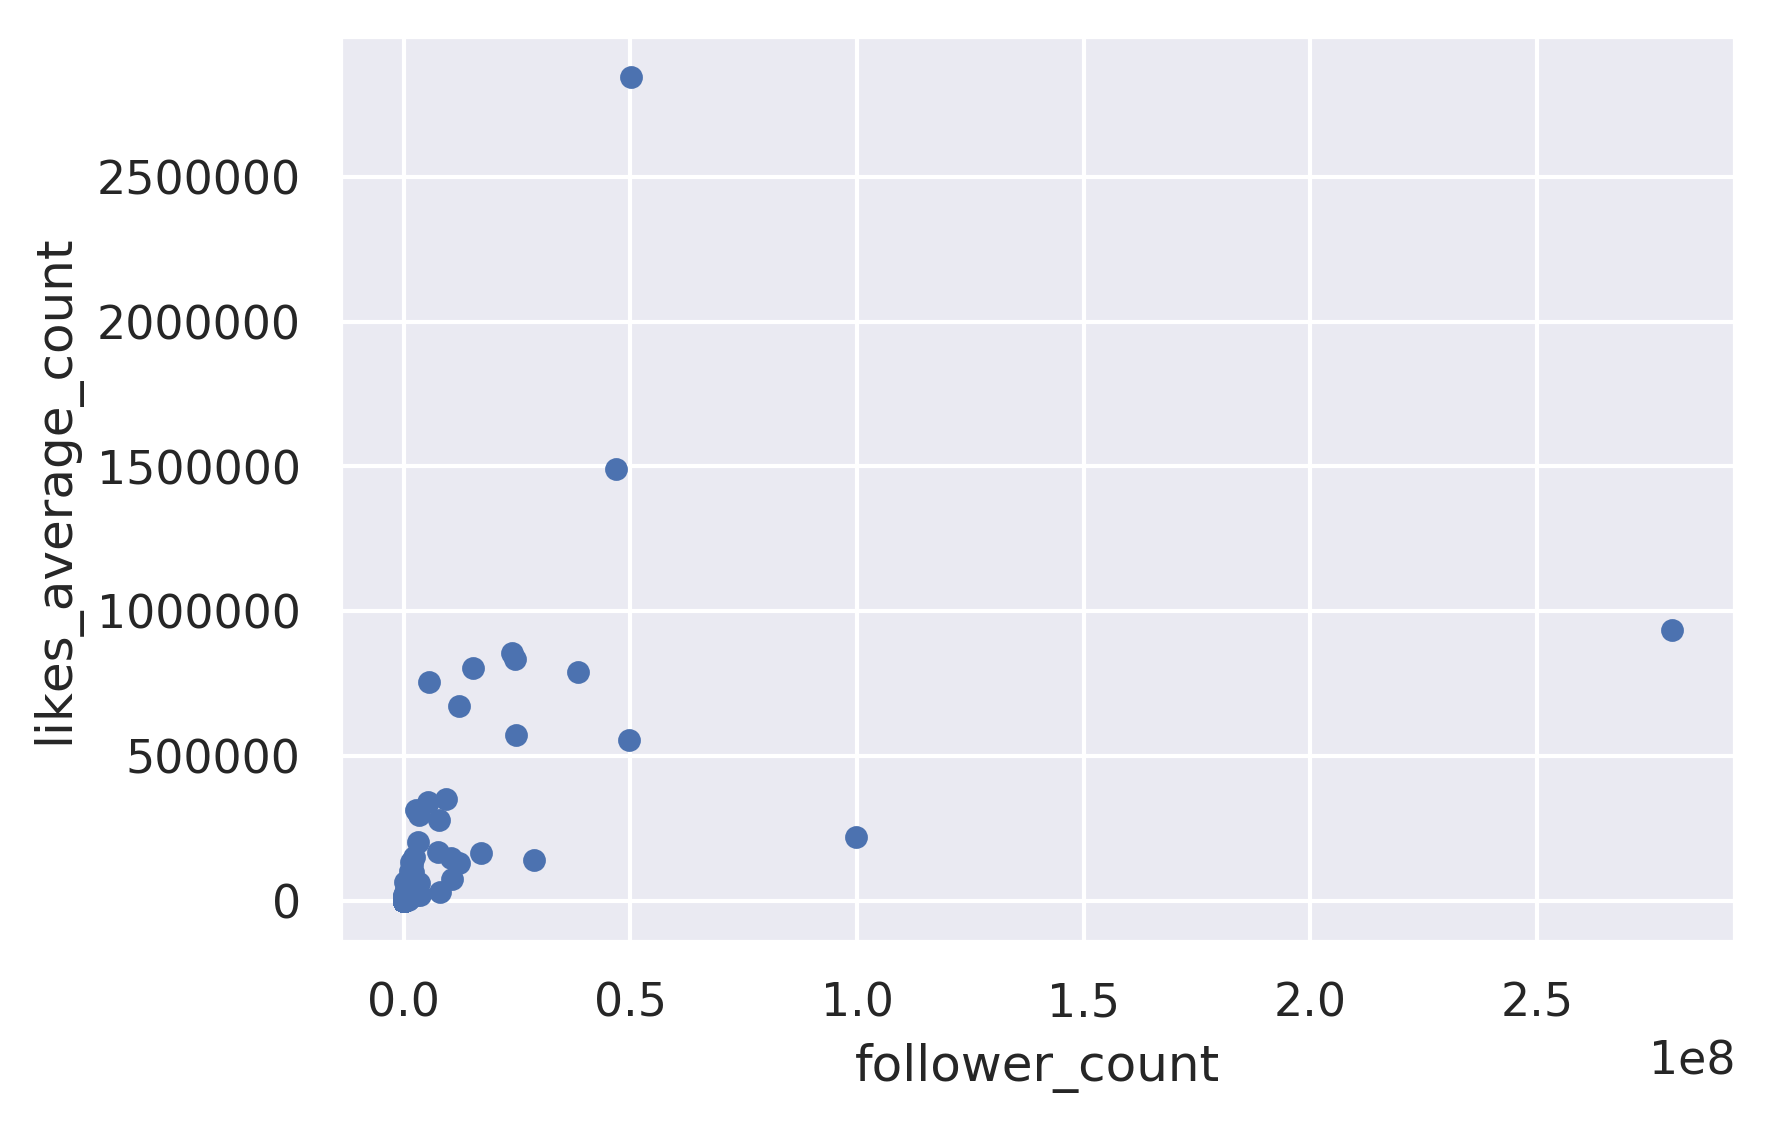
\includegraphics[width=0.75\linewidth]{images/row_data_graph.png}
  \caption{Follower count to average like count plotted}
  \label{fig:raw_data}
\end{figure}

Figure \ref{fig:raw_data} shows that there are some anomalies in the data caused due to disproportionate amount of followers and likes large accounts ran by corporations such as @9gag. Hence, we specify the range of our dataset to be $\mathit{follower\_count} < 10,000$, and $\mathit{likes\_average\_count} < 5000$ to ensure that the these values are within normal range. After the processing is done, Figure \ref{fig:processed_data} shown below is obtained. Much more pleasant. \\

\begin{figure}[h!]
  \center
  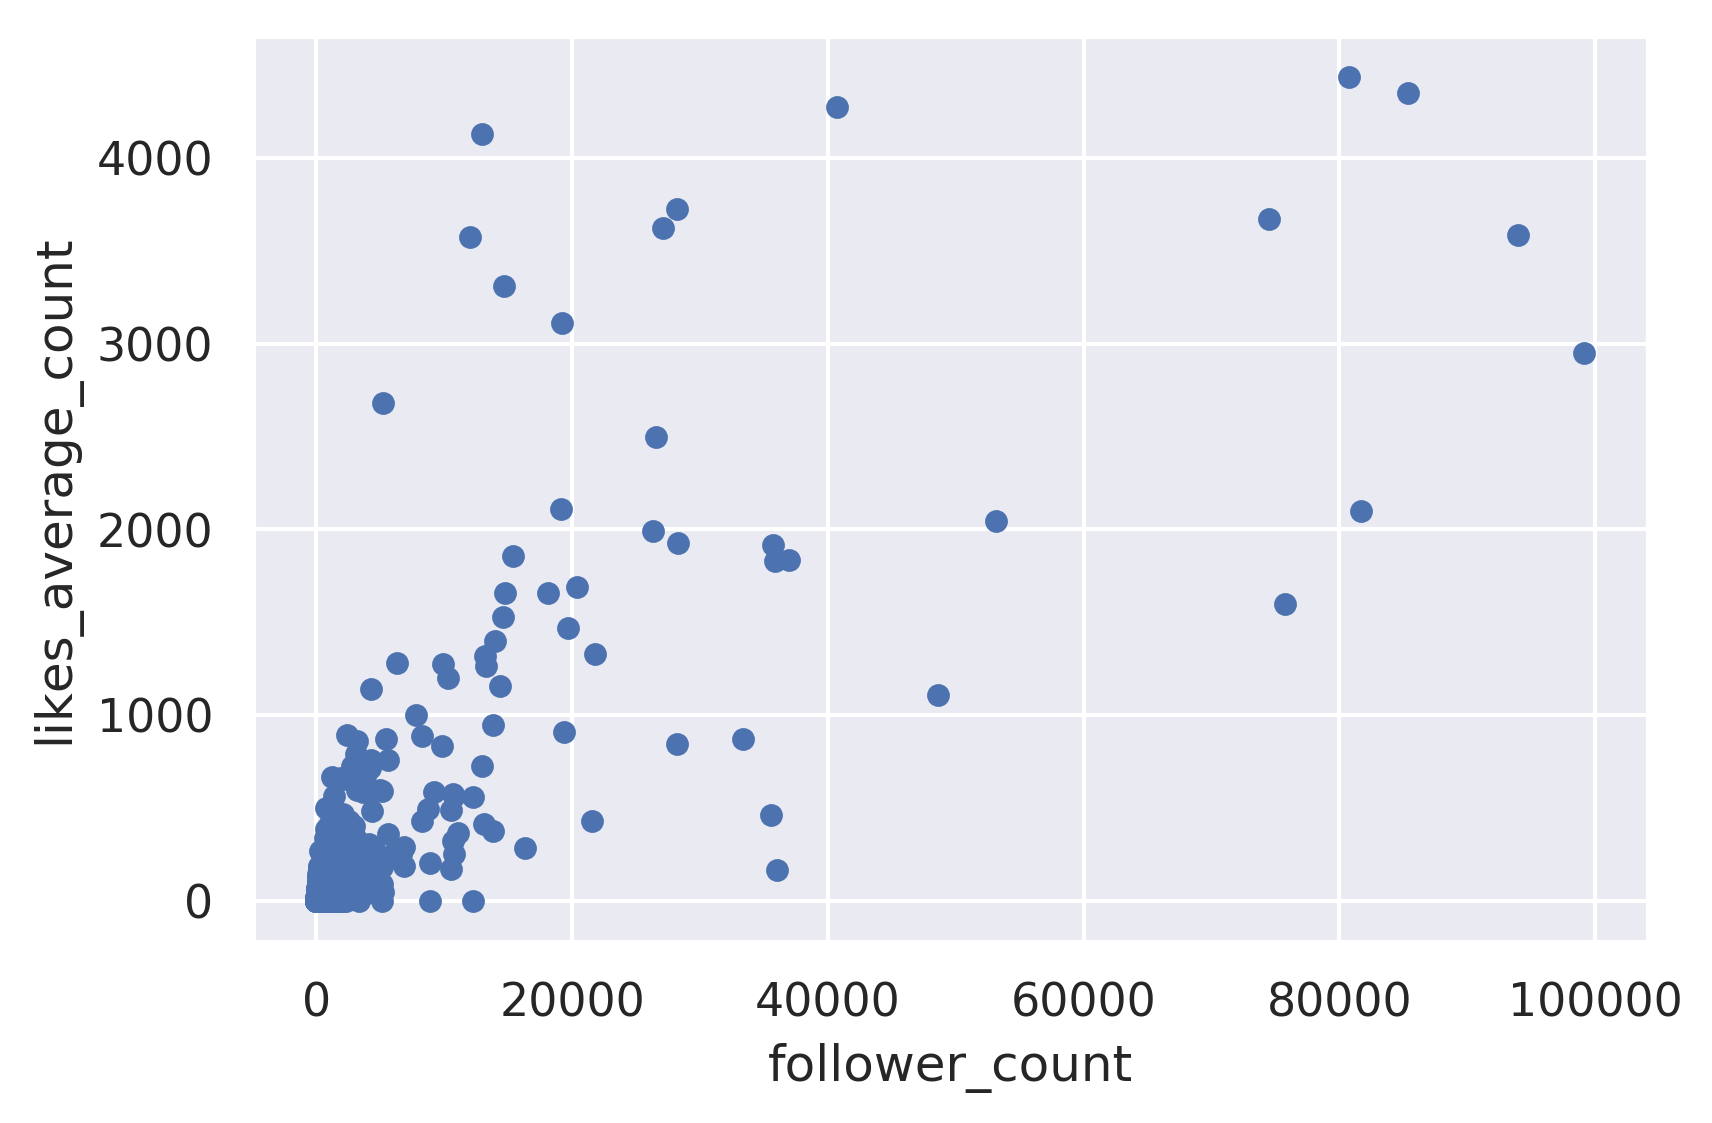
\includegraphics[width=0.75\linewidth]{images/processed_data_graph.png}
  \caption{Follower count to average like count plotted}
  \label{fig:processed_data}
\end{figure}

Additionally, as the distribution of data appears skewed, a logarithmic scale will be used to normalise the distribution. The graph we obtain is shown below ( \ref{fig:log_data}).

\begin{figure}[h!]
  \center
  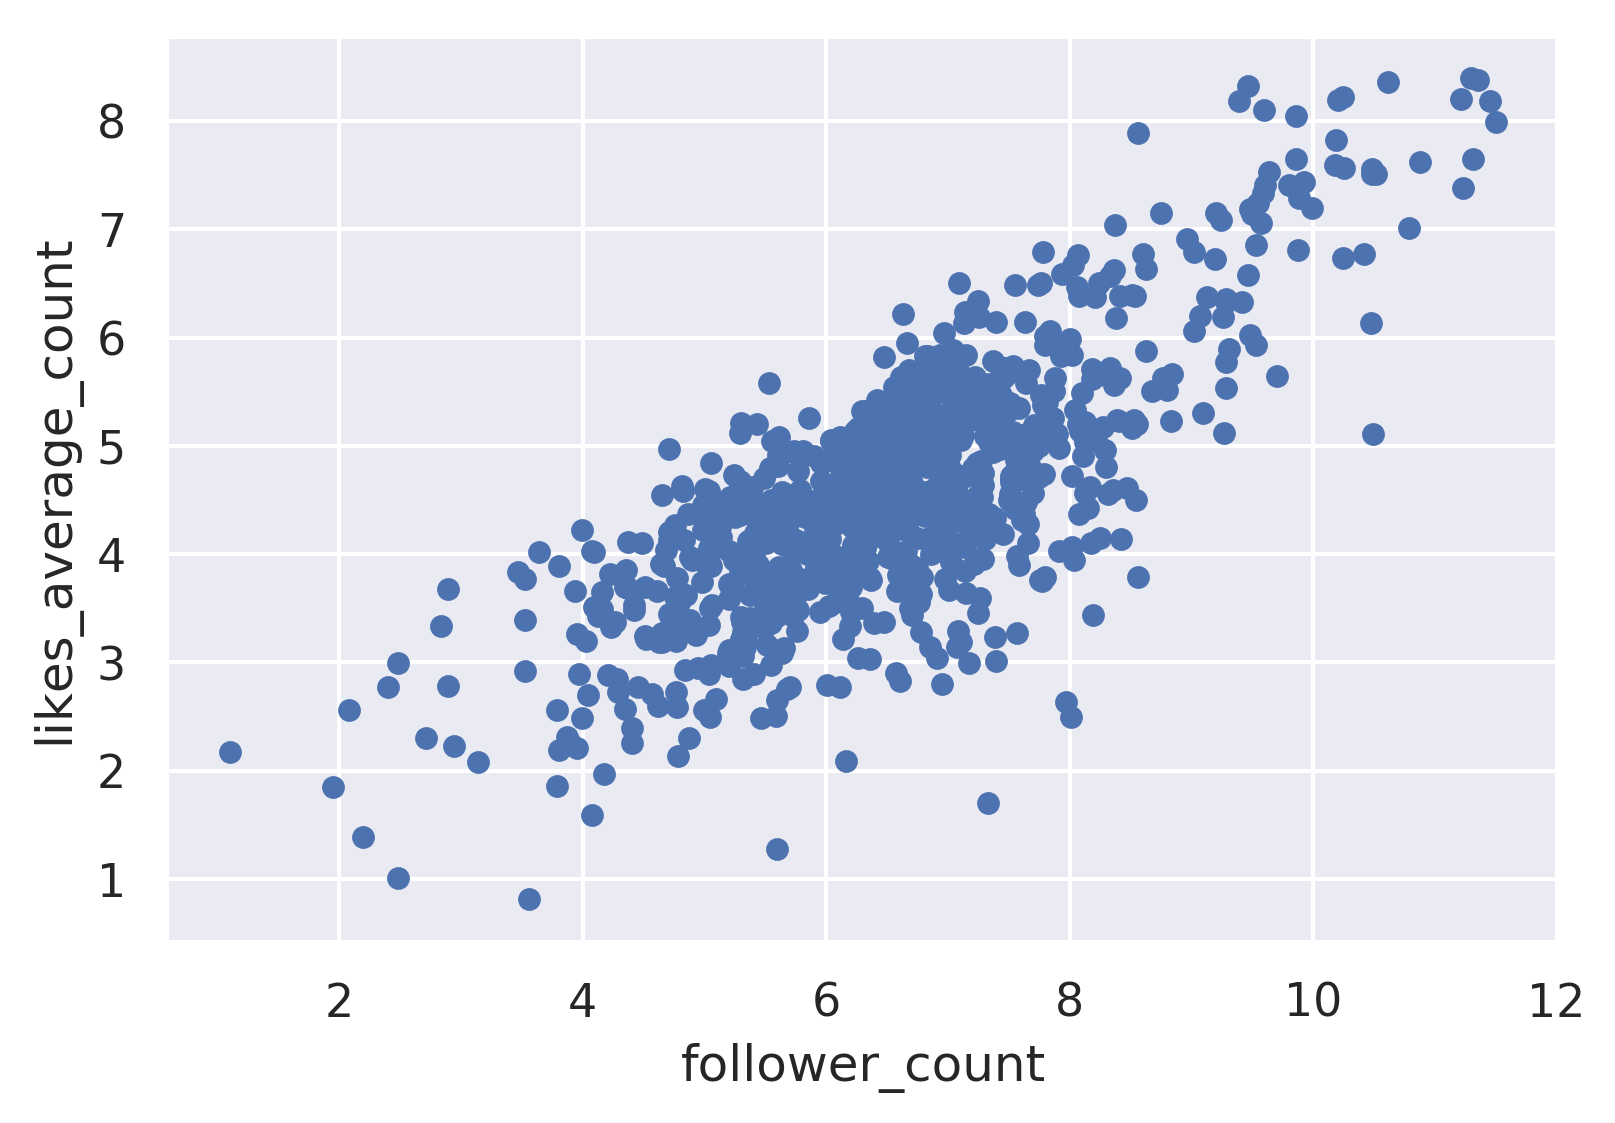
\includegraphics[width=0.75\linewidth]{images/log_data_graph.png}
  \caption{Follower count to average like count plotted}
  \label{fig:log_data}
\end{figure}

\section{Analysis}\label{section-analysis}

\subsection{Variable Definition}
For formality purposes, the following definition will be used for the natural logs of two values:

$x=\ln{\mathit{follower\_count}}, y=\ln{\mathit{likes\_average\_count}}$

Upon counting, the number of variable pairs $ \left( x _ { i }, y _ { i } \right)$ is found to be $872$, and hence, 

\begin{align}
{n = 872}
\end{align}

\subsection{Value Calculation}
First, to calculate the sample mean value for both variables like count $x$, follower count $y$
\begin{align}
\overline { x } = \frac { 1 } { n } \sum _ { i = 1 } ^ { n } x _ { i } = \frac { 1 } { 872 } (5.04 + 3.81 + \ldots + 11.2 + 6.59)  { = 4.58}
\end{align}
\begin{align}
\overline { y } = \frac { 1 } { n } \sum _ { i = 1 } ^ { n } y _ { i }  = \frac { 1 } { 872 } (4.06 + 2.19 + \ldots + 7.37 + 3.98)  {= 6.57}
\end{align}
In analysing the relationship between the two variables, it is beneficial to derive the Pearson's coefficient as the following between $x$ and $y$
\begin{align}
r _ { x y } &= \frac { \sum _ { i = 1 } ^ { n } \left( x _ { i } - \overline { x } \right) \left( y _ { i } - \overline { y } \right) } { \sqrt { \sum _ { i = 1 } ^ { n } \left( x _ { i } - \overline { x } \right) ^ { 2 } } \sqrt { \sum _ { i = 1 } ^ { n } \left( y _ { i } - \overline { y } \right) ^ { 2 } } } \\
r _ { x y } &= \frac {\left( 154 - 230 \right) \left( 3222 - 2801\right)  + \ldots + {\left( 320 - 230 \right) \left( 840 - 2801\right) }}  { \sqrt { \left( 154 - 230\right) ^ { 2 }  + \ldots +  \left( 3222 - 2801\right)^{2}} \sqrt { \left( 320 - 230\right) ^ { 2 }  + \ldots +  \left( 840 - 2801\right)^{2}} } \\
r _ { x y } &=
\end{align}

\section{Experiments}\label{section-experiments}

\section{Conclusions}\label{section-conclusions}

\section{Sample}\label{section-sample}

\section{Appendix}\label{section-appendix}



\bibliographystyle{apacite}
\bibliography{instagram}

\end{document}